%%%%%%%%%%%%%%%%%%%%
% Background of ecPoint-Rainfall testers

\section{Background}
\begin{figure}
\centerline{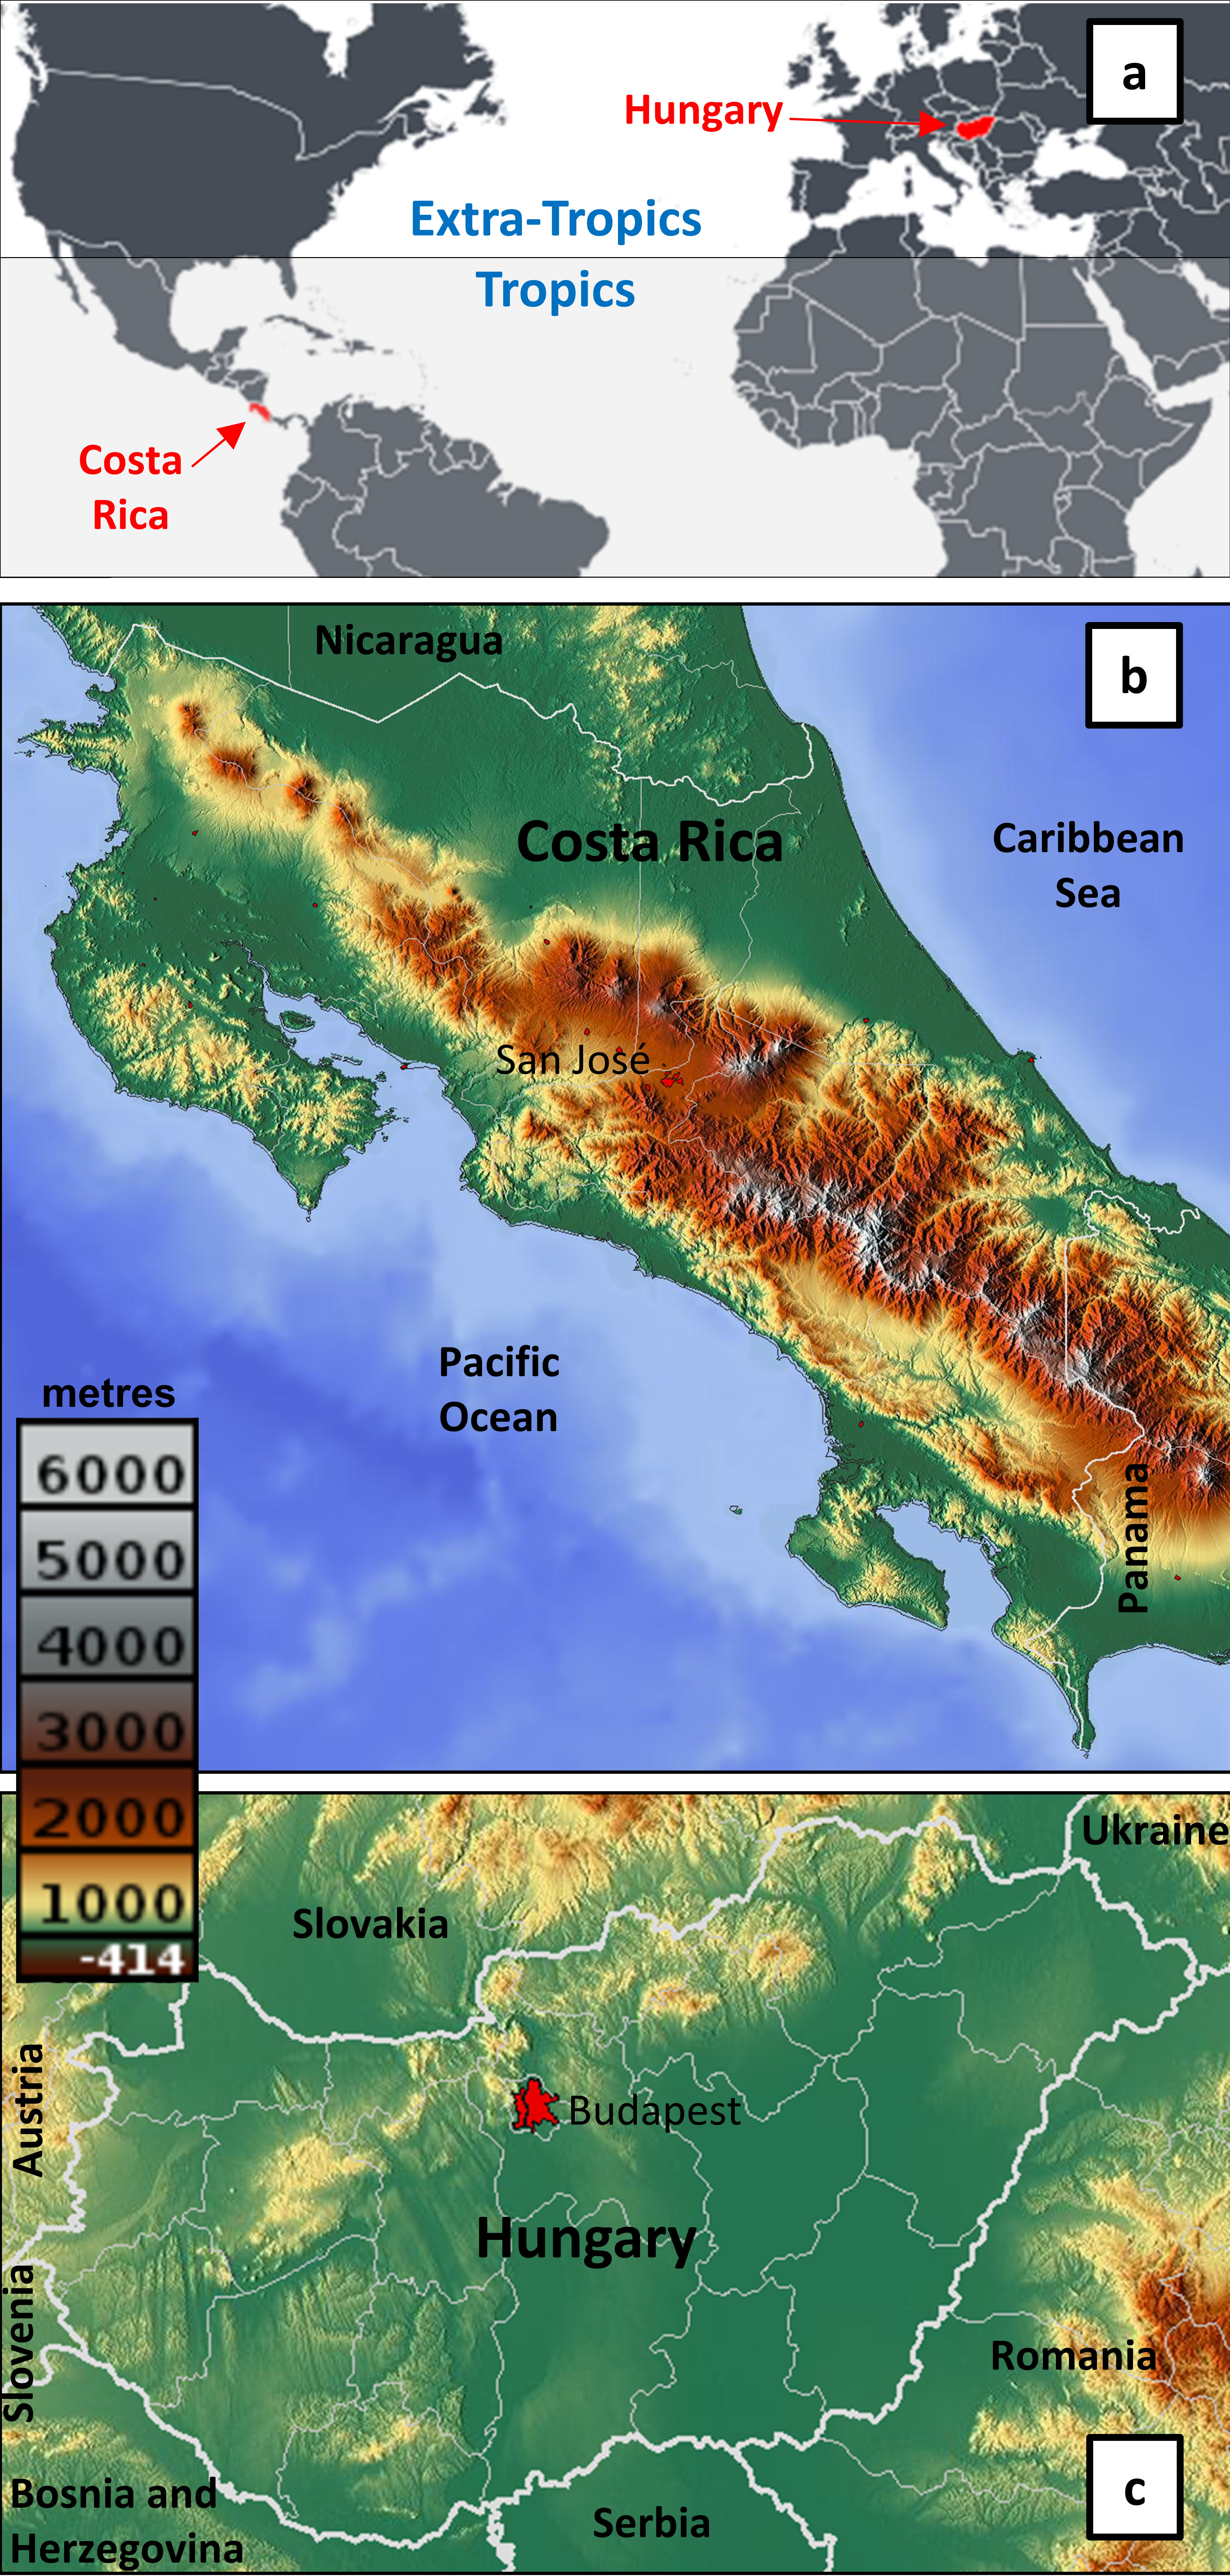
\includegraphics[width=19pc]{manuscript/Figures/Background_Location_H_CR.png}}
\caption{Panel (a) shows Costa Rica location in Central America and Hungary location in Europe. Panel (b) and (c) show respectively the orography of Costa Rica and Hungary.}
\label{GeoLocation_H_CR}
\end{figure}

\subsection{How does IMN forecast extreme rainfall?}
At IMN, extreme rainfall predictions mostly rely on deterministic systems. From the Weather Research and Forecasting (WRF) system, IMN has developed a series of model versions (WRF-1.5, WRF-5, WRF-AR, WRF-Sarapiquí, WRF, WRF-8, WRF-15) with different spatial/temporal resolutions, domains, and model configurations to tailor their use for specific hazards (e.g. tropical waves, tropical cyclones, cold fronts, hail, and forest fires). In particular, WRF-1.5, developed in 2018, produces forecasts at 1.5 km resolution, up to 5 days, and aims to improve predictions for convective systems which generally tend to produce extreme localized rainfall in Costa Rica.\par
IMN also works with EPFs, although its experience is relatively recent. IMN mostly works with the Global Forecast System (GFS) developed by the National Centers for Environmental Prediction in the USA. Still, from 2018, it started also using the ECMWF ENS.

\subsection{How does OMSZ forecast extreme rainfall?}
OMSZ has a long-standing experience (since the 1990s) in developing, using, and verifying EPFs. Therefore, extreme rainfall predictions are mostly generated and disseminated to the public using EPFS. OMSZ forecasters would typically look at a suite of ensemble models, including AROME, ALADIN and ECMWF. OMSZ forecasters also take part regularly in educational and training programmes about the ECMWF ENS to keep updated on ensemble developments and improve the use of ECMWF probabilistic products.\par
OMSZ is also experienced in rainfall post-processing which is regularly used at OMS to add value in the forecast of small-scale low-predictability phenomena like extreme localized rainfall \citep{Ihasz2018, Matrai2017}.



